%!TEX root = informe.tex

\subsection{Pseudocódigo relevante a los métodos de interpolación}
\par \IEEEPARstart{A}{} continuaci\'on nos explayaremos sobre los detalles de
implementaci\'on de cada m\'etodo propuesto.

\vspace{0.4cm}

$$f(x) = a + b (x - x_0)$$

$$y_0 + (y_1-y_0) \times \frac{x - x_0}{x_1 - x_0} \implies a = y_0 \ \wedge \ b = \frac{y_1-y_0}{x_1-x_0}$$

\begin{algorithm}
    \KwIn{Puntos del dominio conocidos $x$ ; Puntos de im\'agen conocidos $y$, grado funci\'on $gr$}
    \KwOut{Vector coeficiente $a$, Vector coeficiente $b$}
    
    \For{$i = 1 \ldots gr-1$}
    {		
		$a_i \gets y_i$\;
		$b_i \gets \frac{y_{i+1} - y_{i} }{x_{i+1} - x_{i}}$\;
	}
    \KwRet{$a$,$b$}
    \caption{Pseudoc\'odigo del algoritmo de Interpolaci\'on lineal}
    \label{alg:int_lineal}
\end{algorithm}

$$f(x) = d + c ( x - x_0 ) + b ( x - x_0)^2 + a ( x - x_0)^3$$

\begin{algorithm}
    \KwIn{Puntos del dominio conocidos $x$ ; Puntos de im\'agen conocidos $y$, grado funci\'on $gr$}
    \KwOut{Vector coeficiente $a$, Vector coeficiente $b$, Vector coeficinete $c$, Vector coeficiente $d$}
    
	$MatrizSplines(0,0) \gets  1$\;
	$MatrizSplines(1,0) \gets  0$\;
	$vectorIndep_0 \gets 0$\;    
    
    \For{$i = 2 \ldots gr-1$}
    {		
		$MatrizSplines(i,i-1) \gets x_i - x_{i-1}$\;
		$MatrizSplines(i,i) \gets 2 \ (x_{i+1} - x_{i-1})$\;
		$MatrizSplines(i,i+1) \gets (x_{i+1} - x_i)$\;
		$vectorIndep_i \gets 3 \  \frac{y_{i+1} - y_i }{x_{i+1}- x_{i}} - \frac{y_i - y_{i-1}}{ x_i -x_{i-1}}$\;
	}    
	
	$MatrizSplines(gr,gr) \gets  1$\;
	$MatrizSplines(gr,gr-1) \gets  0$\;
	$vectorIndep_{gr} \gets 0$\; 
	
	$b \gets ResolverSistemaEcuaciones(MatrizSplines,vectorIndep)$\;
	
	\For{$i = 1 \ldots gr$}
	{
		$a_i \gets \frac{1}{3 \ \frac{b_{i+1} - b_{i}}{x_{i+1} - x_i}}$\;
		$b_i \gets \frac{y_{i+1}- y_i}{x_{i+1}- x_i} - \frac{1}{3 \ (2 \ b_i + b_{i+1}) * (x_{i+1} - x_{i})}$\;
	}    
	
	$y \gets d$	
	
    \KwRet{$a$,$b$,$c$,$d$}
    \caption{Pseudoc\'odigo del algoritmo de Interpolaci\'on por Splines}
    \label{alg:int_splines}
\end{algorithm}


El algoritmo de vecino mas cercano es simplemente copiar los frames apropiadamente como se explicó en la sección Desarrollo.

\subsection{Diseño del programa}
Desde un punto de vista de diseño, se explicarán brevemente las decisiones tomadas acerca de estructuras de datos y flujo de datos desde el video de input hasta el video de output. Se mencionarán además, posibles mejoras que quedaron fuera de este trabajo por cuestiones de tiempo.

\emph{Nota}: Se ignorarán partes del programa hechas específicamente para la experimentacion, centrándonos únicamente en el efecto de slowmotion sobre un video de entrada.

Se tienen los siguientes renombres y estructuras:
\begin{itemize}
	\item \texttt{Pixel}: Byte sin signo.
	\item \texttt{Frame}: Conjunto ordenado en 2 dimensiones de \texttt{Pixel}es.
	\item \texttt{Video}: Metadata del video\footnote{Ancho, Alto, fps, Cantidad de frames.} y un conjunto ordenado de \texttt{Frame}s.
\end{itemize}

Representamos los conjuntos ordenados como arreglos, utilizando el contenedor \texttt{vector} de la libreria STL de C++.

Explicaremos en órden de procesamiento las etapas del flujo de datos:
\begin{enumerate}
    \item Lectura del video de disco a RAM: se utilizó la librería \emph{OpenCV} para leer un video desde un stream y guardarlo en una estructura \texttt{Video} mencionada anteriormente. Se lee el video completo a RAM, convirtiendolo a escala de grises mediante una función provista por la librería\footnote{La conversión de color de escala de grises a RGB consiste en replicar la intensidad de brillo en cada componente de color\cite{grayscale}.}
	\item Se procesa el video según el método de interpolación elegido y sus parámetros asociados. En caso de interpolación lineal o vecino más cercano, simplemente se itera entre todos los pares de \texttt{Frame}s consecutivos generando segun corresponda los \texttt{Frame}s intermedios. En el caso de splines, se divide el \texttt{Video} en bloques de un tamaño determinado por parámetro y se genera un spline para cada \texttt{Pixel} dentro de cada bloque. Luego, se procede a generar \texttt{Frame}s intermedios evaluando estos splines para cada \texttt{Pixel} en el punto intermedio correspondiente.
	\item Finalmente, se realiza el proceso opuesto con \emph{OpenCV}: se escribe desde una estructura \texttt{Video} a una stream binario con un formato de video determinado.
\end{enumerate}

\begin{figure}[h!]
  \begin{centering}
    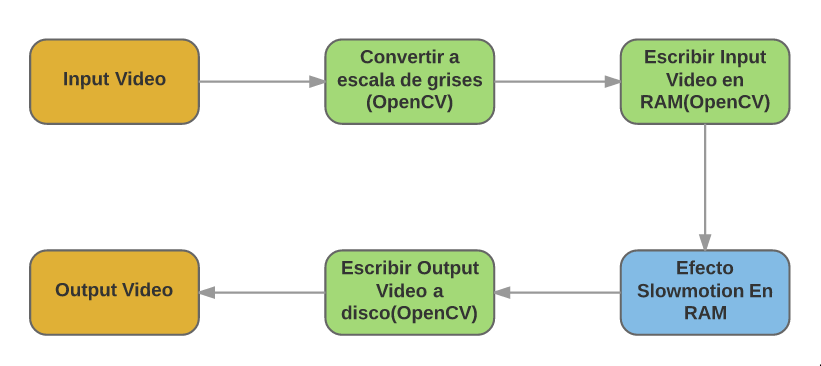
\includegraphics[width=0.55\textwidth]{img/dataflow.png}
     \caption{Flujo de procesamiento de datos del video}\label{fig:dataflow}
 \end{centering}
\end{figure}

Como posibles mejoras se tienen:
\begin{itemize}
	 \item Leer el video de forma \emph{lazy} y escribir de forma \emph{golosa}, es decir, leer de disco a RAM únicamente el conjunto de frames necesarios para trabajar\footnote{El tamaño de bloque spline en interpolación spline, o 2 píxeles en los otros métodos.}, generar nuevos frames e ir escribiéndolos al resultado a medida que se generan. Esto minimizaría el uso de la memoría RAM respecto a la solución actual que mantiene todo el video de input y output en RAM antes de escribir a disco.

	 \item Aprovechar la forma tridiagonal de la matriz del sistema lineal que queda al resolver un spline utilizando una matriz esparsa, y/o alguna factorización apropiada, para reducir la complejidad temporal y espacial del último método.
\end{itemize}



